\subsection{\label{sub:\projectname-AperB} \textsf{AperB}}

\paragraph{Símbol}

\begin{center} \bsfsymbol{AperB} \end{center}

\paragraph{Entrades i sortides}

\begin{where}
\item[\nodenamebit{sigA}] Signe del primer factor
\item[\nodenamerange{A}{3}{0}] Mòdul del primer factor (BCD)
\item[\nodenamebit{sigB}] Signe del segon factor
\item[\nodenamerange{B}{3}{0}] Mòdul del segon factor (BCD)
\item[\nodenamebit{sigAxB}] Signe del producte
\item[\nodenamerange{AxB}{7}{0}] Mòdul del producte (BCD)
\end{where}

\paragraph{Funció}

Multiplicador BCD d'una xifra amb signe, amb resultat en dues xifres.

Retorna a les sortides $sigAxB$ i $AxB$ el signe i mòdul del producte de $sigA$, $A$ amb $sigB$, $B$.

\paragraph{Inespecificacions}


La sortida no està definida si $A$ o $B$ no pertanyen al seu codi.


\paragraph{Implementació}

\vhdlisting{AperB}

\begin{contendfig}
  \begin{center}
    \adjustbox{max width=\textwidth, max height=\textheight}{
      \bdfschematic{AperB}
    }
  \end{center}
  \caption{\label{fig:sch-\projectname-AperB} Esquemàtic per al bloc \textsf{AperB}}
\end{contendfig}

L'esquemàtic del bloc es pot veure a la figura~\ref{fig:sch-\projectname-AperB} (pàgina~\pageref{fig:sch-\projectname-AperB}).

Es fa servir \textsf{MULT\_8x8} per a dur a terme la multiplicació del mòdul
(els factors son també binari natural), i el resultat es converteix
de binari natural a BCD de dues xifres mitjançant \textsf{CA2\_BCD\_8B},
abans de ser retornat a $AxB$.

Per a calcular el signe del producte es fa servir una \textsf{XOR} entre els
dos signes d'entrada.

\paragraph{Simulació}

\begin{contendfig}
  \begin{center}
    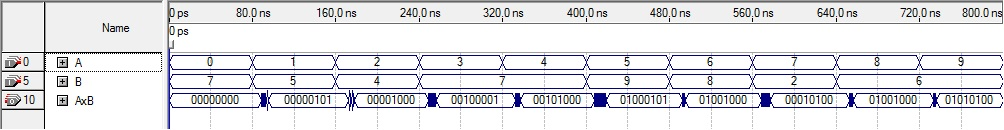
\includegraphics[scale=0.55]{../\projectname/assets/vwf/AperB.jpg}
  \end{center}
  \caption{\label{fig:sim-\projectname-AperB} Simulació per al bloc \textsf{AperB}}
\end{contendfig}

La simulació del bloc es pot veure a la figura~\ref{fig:sim-\projectname-AperB} (pàgina~\pageref{fig:sim-\projectname-AperB}).

% FIXME

\vspace{1cm}
